\section{Геометрический смысл частных
производных, дифференцируемость, дифференциал. касательная на
плоскости.}

\hypertarget{ux447ux430ux441ux442ux43dux44bux435-ux43fux440ux43eux438ux437ux432ux43eux434ux43dux44bux435}{%
\subsection{\texorpdfstring{\textbf{Частные производные}
}{Частные производные }}\label{ux447ux430ux441ux442ux43dux44bux435-ux43fux440ux43eux438ux437ux432ux43eux434ux43dux44bux435}}

Пусть функция $z = f(x,\ y)\ $определена в некоторой области $D$ на
плоскости $xOy$. Возьмем внутреннюю точку $(x,\ y$\emph{)} из
области $D$ и дадим $x$ приращение $\Delta x$ такое, чтобы точка
$\left( x + \Delta x,\ y \right) \in D$. Величину
$\Delta_{x}z = f\left( x + \Delta x,y \right) - f(x,\ y)$ назовем
частным приращением функции $z$ по \emph{x.} Составим отношение
$\frac{\Delta_{x}z}{\delta x}$\emph{.} Для данной точки $(x,\ y)$
это отношение является функцией $\delta x$\emph{.}

\textbf{Определение.} Если при $\delta x \rightarrow 0$ отношение
$\frac{\Delta_{x}z}{\delta x}$ имеет конечный предел, то этот предел

называется частной производной функции $z = f(x,\ y)$ по независимой
переменной \emph{x} в точке

$(x,\ y)$ и обозначается символом $\frac{\partial z}{\partial x}$
(или $f^{'}(x,\ y)$,или $z_{x}^{'}(x,\ y)$). Таким образом, по
определению
$\frac{\partial z}{\partial x}\ \lim_{\delta x \rightarrow 0}\frac{\Delta_{x}z}{\delta x}\ $или,
что то же самое,
$f_{x}^{'}\left( x,y \right) = \lim_{\delta x \rightarrow 0}\frac{f\left( x + \delta x,y \right) - f\left( x,y \right)}{\delta x}\ $.

Если $u = f(x_{1},\ x_{2},\ldots,\ x_{n})$ -- функция $n$
независимых переменных,

то
$\frac{\partial u}{\partial x_{k}} = \lim_{\Delta x_{k} \rightarrow 0}\frac{f\left( x_{1},\ x_{2},..,x_{k - 1} + \Delta x_{k} \right) - f\left( x_{1},\ x_{2},..,x_{k - 1},\ \ \ x_{k},..,x_{n} \right)}{\delta x}$

Заметив, что $\Delta_{x}z$ вычисляется при неизменном значении
переменной $y$, а $\Delta_{Y}z$ -- при

неизменном значении переменной $x$, определения частных производных
можно

сформулировать так: частной производной по $x$ функции
$z = f(x,\ y)$ называется обычная

производная этой функции по $x$, вычисленная в предположении, что
$y$ \emph{--} постоянная;

Частной производной по $y$ функции $z = f(x,\ y)$ называется ее
производная по $y$, вычисленная в предположении, что$\ x$ --
постоянная. Отсюда следует, что правила вычисления частных производных
совпадают с правилами, доказанными для функции одной переменной.

\hypertarget{ux433ux435ux43eux43cux435ux442ux440ux438ux447ux435ux441ux43aux438ux439-ux441ux43cux44bux441ux43b-ux447ux430ux441ux442ux43dux44bux445-ux43fux440ux43eux438ux437ux432ux43eux434ux43dux44bux445-ux444ux443ux43dux43aux446ux438ux438-ux434ux432ux443ux445-ux43fux435ux440ux435ux43cux435ux43dux43dux44bux445.}{%
\subsection{\texorpdfstring{\textbf{Геометрический смысл частных
производных функции двух
переменных.}}{Геометрический смысл частных производных функции двух переменных.}}\label{ux433ux435ux43eux43cux435ux442ux440ux438ux447ux435ux441ux43aux438ux439-ux441ux43cux44bux441ux43b-ux447ux430ux441ux442ux43dux44bux445-ux43fux440ux43eux438ux437ux432ux43eux434ux43dux44bux445-ux444ux443ux43dux43aux446ux438ux438-ux434ux432ux443ux445-ux43fux435ux440ux435ux43cux435ux43dux43dux44bux445.}}

Пусть в трехмерном пространстве поверхность \emph{S} задана уравнением
$z = f(x,\ y)$\emph{,} где $f(x,\ y)$ --

функция, непрерывная в некоторой области \emph{D} и имеющая там частные
производные по \emph{x} и

по \emph{y.} Выясним геометрический смысл этих производных в точке
$M_{0}(x_{0},\ y_{0}) \in D$, которой на

поверхности $z = f\left( x,\ y \right)$ соответствует точка
$N_{0}(x_{0},\ y_{0},\ f(x_{0},\ y_{0})).$

При нахождении частной производной $\frac{\partial z}{\partial x}$ в
точке $M_{0}$ мы полагаем, что $z$ является только

функцией аргумента \emph{x}, тогда как аргумент \emph{y} сохраняет
постоянное значение $y = y_{0}$,

то есть $z = f(x,\ y_{0}) = f_{1}(x).$ Функция
$f_{1}\left( x \right)$ геометрически изображается кривой $L$, по
которой поверхность $S$ пересекается плоскостью $y = y_{0}$. В силу
геометрического смысла производной функции одной переменной
$f_{1}^{'}(x_{0}) = \tan\alpha$\emph{,} где $\alpha$ - угол,
образованный касательной к линии $L$ в точке $N_{0}\ $ с
положительным направлением оси $Ox$\emph{.}

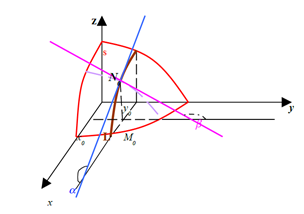
\includegraphics[width=3.21631in,height=2.24359in]{23img.png}

Но
$f_{1}^{'}\left( x_{0} \right) = \left. \ \left( \frac{\partial z}{\partial x} \right) \right|\left( x_{0},y_{0} \right)$
так что
$\left. \ \left( \frac{\partial z}{\partial x} \right) \right|_{M_{0}} = \tan\alpha$

Таким образом, частная производная
$\left. \ \left( \frac{\partial z}{\partial x} \right) \right|_{M_{0}}$
равна тангенсу угла a между осью $Ox$ и

касательной в точке \emph{N0} к кривой, полученной в сечении поверхности
$z = f(x,\ y)$ плоскостью $y = y_{0}$ . Аналогично получаем, что
$\left. \ \left( \frac{\partial z}{\partial y} \right) \right|_{M_{0}} = \tan\beta$

\hypertarget{ux434ux438ux444ux444ux435ux440ux435ux43dux446ux438ux440ux443ux435ux43cux43eux441ux442ux44c-ux444ux443ux43dux43aux446ux438ux438-ux43dux435ux441ux43aux43eux43bux44cux43aux438ux445-ux43fux435ux440ux435ux43cux435ux43dux43dux44bux445}{%
\subsection{\texorpdfstring{\textbf{Дифференцируемость функции
нескольких
переменных}}{Дифференцируемость функции нескольких переменных}}\label{ux434ux438ux444ux444ux435ux440ux435ux43dux446ux438ux440ux443ux435ux43cux43eux441ux442ux44c-ux444ux443ux43dux43aux446ux438ux438-ux43dux435ux441ux43aux43eux43bux44cux43aux438ux445-ux43fux435ux440ux435ux43cux435ux43dux43dux44bux445}}

Пусть функция $z = f(x,\ y)$ определена в некоторой области $D$ на
плоскости $xOy$\emph{.} Возьмем

точку $(x,\ y) \in D$ и выбранным значениям $x$ и $y$ дадим любые
приращения $\delta x $и $\delta y$, но такие,

чтобы точка $(x + \delta x,\ y + \delta y) \in D$\emph{.}

\textbf{Определение.} Функция $z = f(x,\ y)$ называется
дифференцируемой в точке $(x,\ y) \in D$, если

полное приращение
$\delta x = f(x + \delta x,\ y + \delta y) - f(x,y)$ этой функции,
отвечающее приращениям $\delta x$\emph{,} $\delta y$ аргументов,
можно представить в виде

\[\delta z = A\delta x + B\delta y + \alpha(\delta x,\ \delta y)\delta x + \beta(\delta x,\ \delta y)\delta y\]

где $A$ и $B$ не зависят от $\delta x$ и $\delta y$ (но вообще
зависят от $x$ и $y$), а
$\alpha(\delta x,\ \delta y)$ и $\beta(\delta x,\ \delta y)$

стремятся к нулю при стремлении к нулю
$\delta x$ и $\delta y$\emph{.}

Если функция $z = f(x,\ y$\emph{)} дифференцируема в точке
$(x,\ y)$\emph{,} то часть $A\delta x + B\delta y$ приращения

функции, линейная относительно $\delta x$ и $\delta y$, называется
\emph{\textbf{полным дифференциалом}} этой

функции в точке $(x,\ y)$ и обозначается символом
$dz$\emph{:}

\[dz = A\Delta x + \beta\Delta y\]

Таким образом, $\delta z = dz + \alpha\delta x + \beta\delta y$
